\section{Practical Implications}

\subsection{Experimental Setup}

{\bf Datasets and models.} We describe the datasets and models we use in the experiments.

{\it Sentiment Analysis:} This dataset includes six tasks: movie review sentiment (MR), sentence subjectivity (SUBJ), customer reviews polarity (CR), question type (TREC), opinion polarity (MPQA), and the Stanford sentiment treebank (SST) tasks.

{For each task, the goal is to categorize sentiment opinions expressed in the text.
We use an embedding layer (with GloVe embeddings\footnote{http://nlp.stanford.edu/data/wordvecs/glove.6B.zip}) followed by an LSTM layer proposed by~\cite{lei2018simple}.
}
%multi-layer perceptron (MLP), LSTM, CNN on all tasks
%We use this task to verify our theoretical results on model capacity and task covariance in real world.

{\it ChestX-ray14:} This dataset contains 112,120 frontal-view X-ray images and each image has up to 14 diseases.
This is a 14-task multi-label image classification problem.
%We treat each label as one task a binary classification problem and formulate it as a 14-task multi-task learning problem.
%This dataset is curated where the labels
%We use the CheXNet model from~\cite{chexnet}, which is a 121-layer convolutional neural network on all tasks.

For all models, we share the main module across all tasks and assign a separate regression or classification layer on top of the shared module for each tasks.



\subsection{Results and Analysis}

\textbf{A metric to determine positive versus negative transfer.}
We propose a simple metric to determine whether multi-task learning performs better than single-task learning.
The metric is as follows.
First, we train 2 single-task models on 2 separate tasks.
We take the prediction accuracy of the two tasks.
Let $\tau$ be a fixed threshold.
If the accuracy of the source task is higher than the accuracy of the target task by $\tau$, then we predict positive transfer.
On the other hand, if the accuracy of the source task is lower than the accuracy of the target task by $\tau$, then we predict negative transfer.

Table \ref{tab:mtl_better_than_stl} shows the results on a sentiment analysis and an image classification task.

\begin{table}
\begin{center}
  \begin{tabular}{c c c c c}
  \toprule
    \multirow{2}{*}{{\bf Threshold}}  & \multicolumn{2}{c}{{\bf Text classification}} & \multicolumn{2}{c}{{\bf ChestX-ray14}} \\
    & Precision &  Recall & Precision &  Recall \\
    \cmidrule(lr){1-1} \cmidrule(lr){2-3} \cmidrule(lr){4-5}
    0.0 & 0.596 & 1.000 & 0.593 & 1.000 \\
    0.1 & 0.756 & 0.388 & 0.738 & 0.462 \\
    0.2 & 0.919 & 0.065 & 0.875 & 0.044 \\	
    0.3 & 1.000 & 0.004 &     - &     - \\
  \bottomrule
  \end{tabular}
\end{center}
\caption{Ablation study on when should use MTL via different source/target task accuracy. Note: For text classification tasks, the source task training data size ranges from 500 to 1,500 and target task training data size is 1000; For ChestX-ray14, the training data size is 10,000.}
\label{tab:mtl_better_than_stl}
\end{table}

\textbf{Multi-task learning provides labeled data efficiency.}
We measure the data efficiency ratio on text classification tasks.
We find that by performing multi-task learning, only 40$\%$ of the data is needed to achieve comparable performance to single-task learning over all six tasks.

\textbf{Covariance alignment provides more improvement when data size is imbalanced.}
We validate that the performance of aligning task covariances depends on the size of source task data.
Recall that the covariance alignment procedure in \cite{WZR20} adds an additional module between the word embedding representation and the shared module.

In Figure \ref{fig_covariate}, we observe that the benefit from aligning task covariances becomes more significant as we increase the size of the source task dataset.

\begin{figure}[!ht]
	\centering
	\begin{subfigure}[b]{0.33\textwidth}
		\centering
		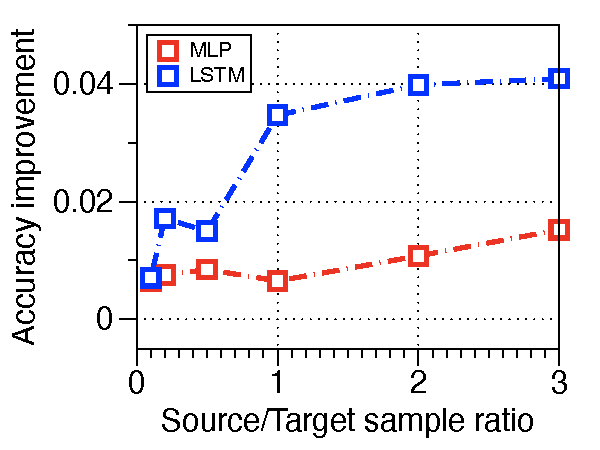
\includegraphics[width=0.975\textwidth]{figures/ratio_alignment_norm_diff_all.pdf}
		\caption{Averaged}
	\end{subfigure}\hfill
	\begin{subfigure}[b]{0.33\textwidth}
		\centering
		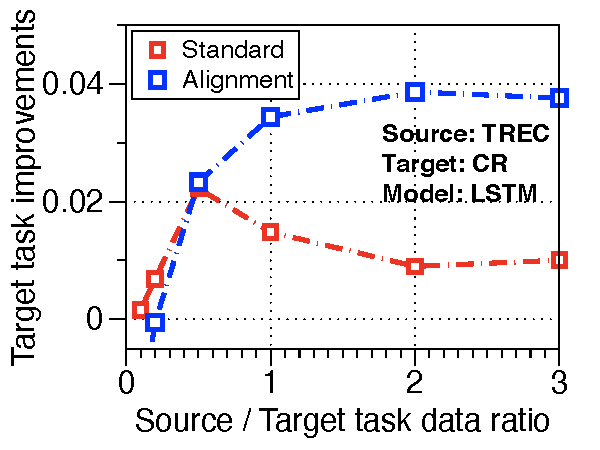
\includegraphics[width=0.975\textwidth]{figures/ratio_alignment_norm_trec_cr_lstm.pdf}
		\caption{Task pair TREC and CR}
	\end{subfigure}\hfill
		\begin{subfigure}[b]{0.33\textwidth}
		\centering
		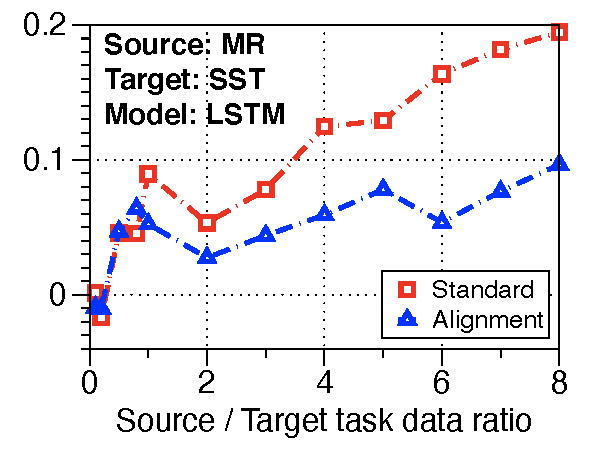
\includegraphics[width=0.975\textwidth]{figures/ratio_alignment_mr_sst_lstm.pdf}
		\caption{Task pair MR and SST}
	\end{subfigure}
	\caption{The performance of aligning task covariances depends on data size. As the ratio between source task data size and target task data size increases, the performance improvement from aligning task covariances increases.}
	\label{fig_covariate}
\end{figure}

%\begin{figure}
%	\centering
%	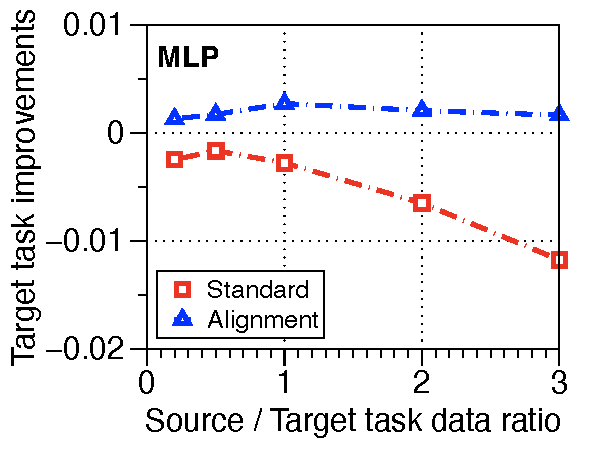
\includegraphics[width=0.5\textwidth]{figures/ratio_alignment_mlp.pdf}
%	\caption{Covariate shift experiment.}
%\end{figure}
